\documentclass[../main.tex]{subfiles}
\begin{document}
	\chapter{Machine Learning} \label{ch:machine}
	

	\section{Machine Learning Basics}
	\noindent 
	
	\noindent  \textit{Machine Learning} focuses on the development of algorithms and models that enable computers to learn from data with the aim of making predictions without being explicitly programmed.\\ \\  
	We can think about learning as the way we understand it as a human. We can classify a learning problem based on the degree of feedback. Machine learning models fall into three primary categories:
	\begin{itemize}
		\item Supervised learning, where we have immidiate feedback.
		\item Reinforcement learning, where we have indirect feedback. For example whenwe are playing the game of chess.
		\item Unsupervised learning, where we have non feedback signal. For example,deducing which dog belongs to each owner.
	\end{itemize}
	Machine learning models simplify reality for the purposes of understanding or prediction. This prediction can be either a numerical prediction or a classifications prediction. 
	A number of machine learning algorithms are commonly used. These include: 
	\subsection{Linear Regression}
	\noindent A linear regression algorithm is used to predict numerical values, based on a linear relationship between different values. A simple linear model has an outcome, denoted by $y$, also known as a response variable,  and a predictor, $x$. It is defined by the following equation.
	
	$$ y_i= \beta_0 + \beta_1 x_i + \epsilon $$

	 \noindent where $ i = 1, ..., n$  indexes the observations from 1 to $n$ in the dataset.

	\begin{figure}[h]
		\centering
		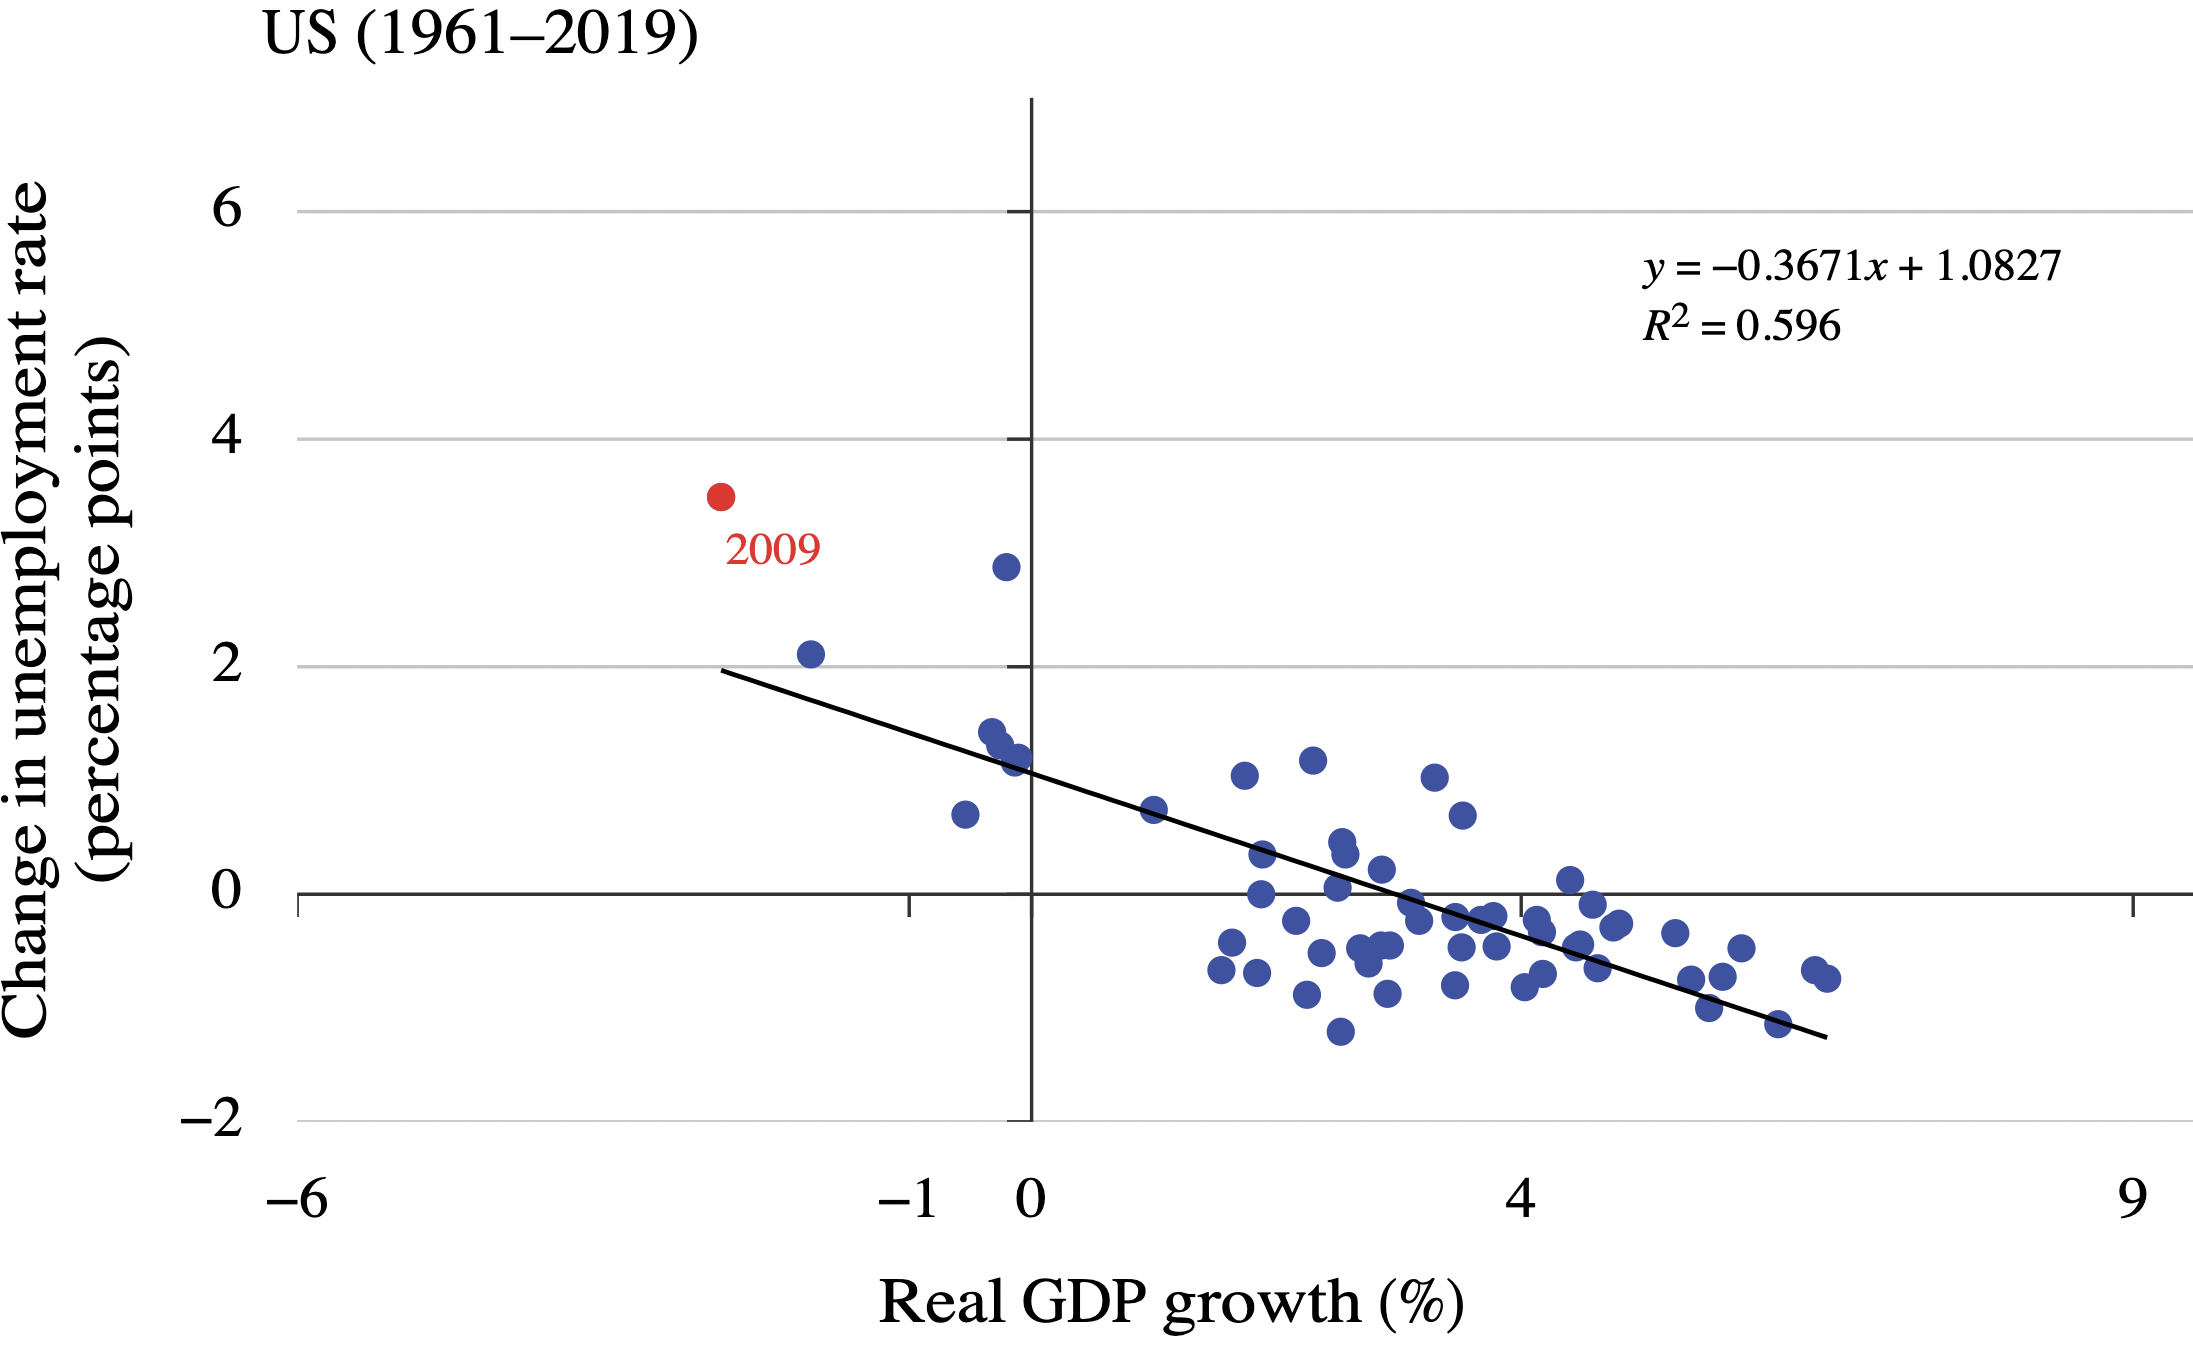
\includegraphics[width=0.6\linewidth]{imgs/gdp.png}
		 \caption{\small $y$ - response variable: unemployment rate , $x$ predictor: GDP growth , } 
	\end{figure} \mbox{} \par

\noindent We can add additional $p$ predictors to a simple linear model, transforming it into a multivariate linear model, which we define as follows:

$$y_i = \beta_0 + \beta_1x_{1i} + \ldots + \beta_px_{pi} + \epsilon_i $$

\subsection{Logistic Regression}
\noindent A logistic regression algorithm is used for classification tasks where the goal is to predict the probability that an instance of belonging to a given class. We need to define the concept of sigmoid function that will be important along te work. \\ \\ A sigmoid function is a mathematical function that maps input values to a range between 0 and 1. We have the following sigmoid function, the logit function: 

\[
\text{logit}: \mathbb{R} \to (0,1)
\quad \text{and is expressed as:} \quad
\text{logit}(x) = \log\left(\frac{x}{x-1}\right)
\]

\noindent The transformed result, $\text{logit}(x)$, is expressed in logarithms of probabilities. The probabilities of the result (also known as odds ratios) can be written as:

\[
P(y_i = 1) = p_i \quad \text{and} \quad \text{logit}(p_i) = x_i \beta
\]

The logistic model can be alternatively written using the inverse logit:

\[
P(y_i = 1 | x_i) = \text{logit}^{-1}(x_i \beta)
\]

\noindent where $y_i$ is the binary response, $\text{logit}^{-1}$ is the inverse logit function, and $x_i \beta$ is the linear predictor.


\subsection{A learning problem}
\noindent Consider the problem of assessing the eligibility of a consumer for a credit. We are provided with the following set of data: \\ 

\begin{tabular}{ll}
	\toprule
	\textbf{Costumer application:}  \\ 
	\midrule
	Age & 23 years \\
	Gender & Male \\
	Annual Salary & \$30,000 \\
	Years in Residence & 1 year \\
	Years in Job & 1 year \\
	Current Debt & \$15,000 \\
	... & ... \\
	\bottomrule
\end{tabular} 
\\ \\
\begin{itemize}
\item Input: \textbf{$x_c=(x_{c_1},...,x_{c_d})$}  "attributes of the costumer that we want to classify". 
\item Output:  
\[
y = \begin{cases}
	approve \\
	deny& \\
\end{cases}
\]

\item Target funtion: $f$  "ideal credit approval formula"
\item Data: The set $\{(x_1, y_1),(x_2,y_2),...,(x_n ,y_n)\}$ corresponds of a historical records of credit customers where $x_i$ is the attributes of the costumer and $y_i$ classification awarded.
\end{itemize}

\noindent We are looking for the function $f$ such that $f(x_c)=y$.
\\ \\ 

	\noindent 
	A fundamental problem of machine learning is the following. Given data of the form $\{(x_i,y_i)\}^m_{i=1} \subset \mathbb{R}^n \times \mathbb{R}$, drawn randomly from a probability distribution $\mu$, find a model P such that $P(x_i)=y_i$. An important aspect of machine learning is that \textit{many supervised learning tasks are about function learning.}. 
\begin{xmpl}
	\noindent An example of a supervised learning task is digit recognition. The objective is to identify handwritten digits (0-9) based on input images. In this task, we aim to learn a probability distribution function denoted as $f$, which maps a set of pixel values ranging from 0 (black) to 255 (white), representing a 28x28 image, to a probability distribution over the digits 0 to 9.

$$f: \{0,..., 255\}^{28 \times 28} \longrightarrow \text{probability distribution on } \{0,1,...,9\}$$

\end{xmpl}
\begin{xmpl} Example of a classification problem. We want to classify if an image is a dog or not a dog. We would like to produce a value which is correlated with the probability of this image being a dog or not a dog.  We can approach the problem in the following way. We want to find a function that takes very high values when dog-image and very low val ues when non dog images and takes the value 0 when its uncertain. 
	$$d: \mathbb{R}^{\# \text{pixels in image}} \rightarrow \mathbb{R} $$
	such that $\mathbb{P}(d(\text{image})) = \text{probability that the image is a dog.}$ \\ \\  
	That is what we mean by many problems can be recast as function learning. Note that there is not a god-given reason why this function should exist. We know that certain points in space, and they have certain values associated to them, but we dont know that there is some big function. 
\end{xmpl}

\noindent \textit{Important principle $II$}: Sometimes function learning can be recast as a classification problem.  
\\ \\ 
Binary classification problem. 
Rather learning $\mu : \mathbb{R}^{\# \text{bits}} \rightarrow \mathbb{R}$ where big values correspond to likely and small values to unlikely. It is better to learn $\mu : \mathbb{R}^{\# \text{bits}} \rightarrow $ probability distribution on $\{-1,0,1\}$. In number theory the function $\mu(n)$ it is called Möebius function 

\[
\mu(n) = \begin{cases}
	0 & \text{if } n \text{ has a repeated square factor}, \\
	-1 & \text{if } n \text{ has an odd number of distinct prime factors}, \\
	1 & \text{if } n \text{ has an even number of distinct prime factors}.
\end{cases}
\]

	
	 
	
\end{document}